%!Tex Root = ../main.tex
% ./Packete.tex
% ./Design.tex
% ./Deklarationen.tex
% ./Vorbereitung.tex
% ./Aufgabe2.tex
% ./Aufgabe3.tex
% ./Aufgabe4.tex
% ./Appendix.tex

\section{Aufgabe 1}

\setcounter{exercise}{1}

\begin{frame}[allowframebreaks]{Aufgabe \thesection}{4-Bit-Carry-Ripple-Addierer, Tiefe}

\begin{solution}
    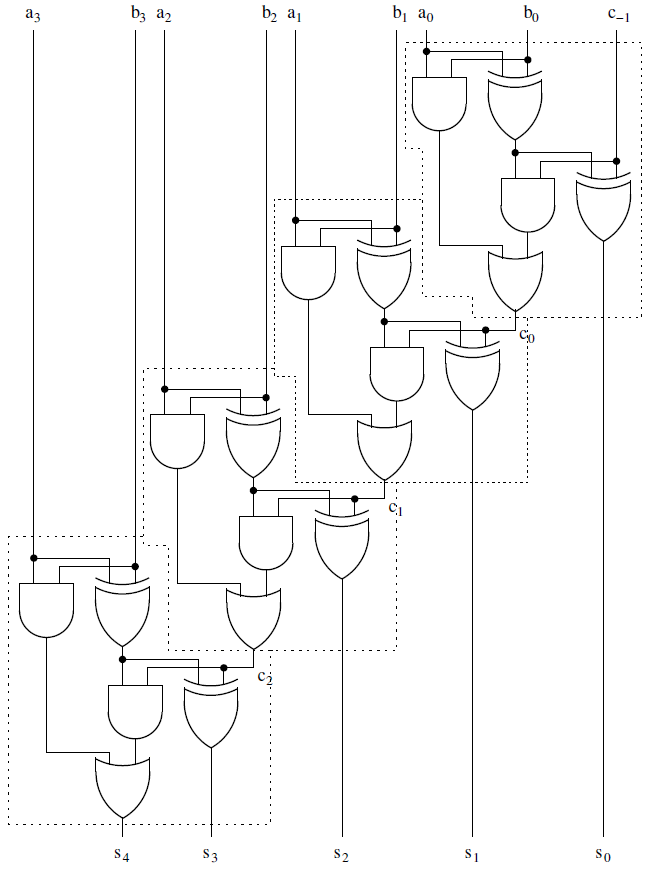
\includegraphics[height=0.5\paperheight, center]{content/CRA.png}
\end{solution}

\begin{solution}
    \begin{itemize}
        \item Allgemein gilt $depth(CR_n) = 3 + 2(n - 1)$. Hier: $depth(CR_4) = 3 + 2(4 - 1) = 9$ \end{itemize}
    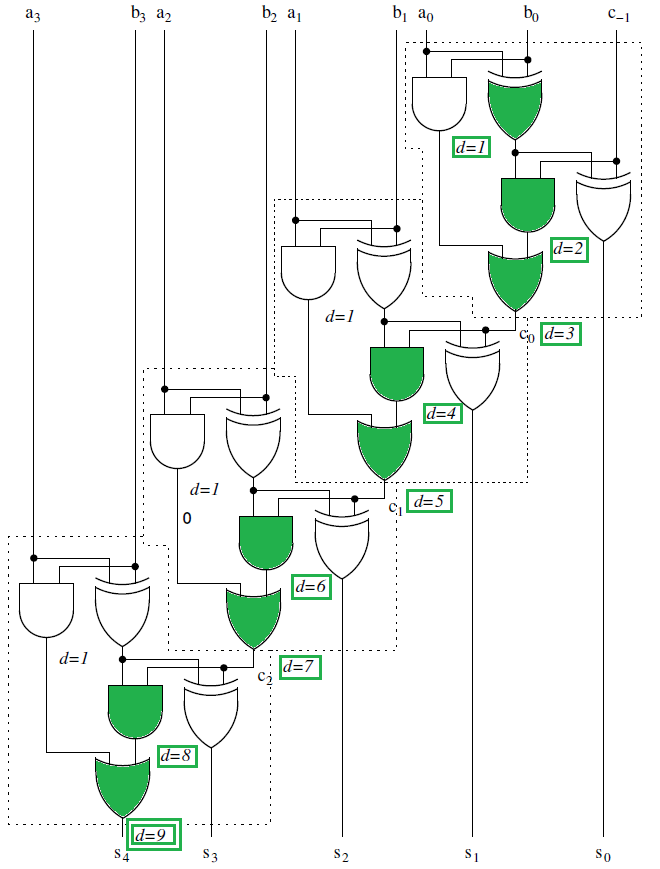
\includegraphics[height=0.5\paperheight, center]{content/CRA-Depth.png}
\end{solution}

\begin{solution}
    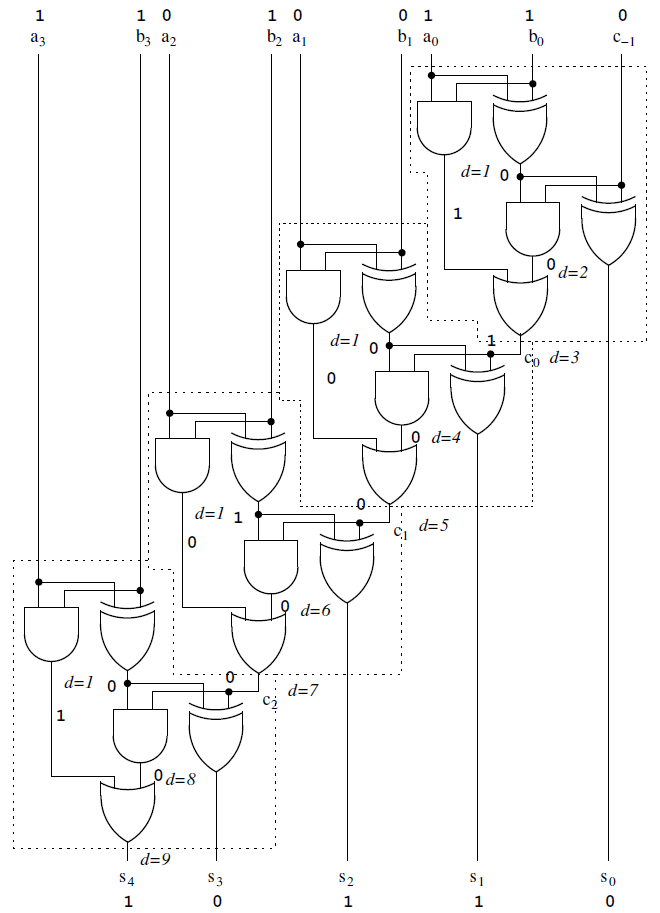
\includegraphics[height=0.5\paperheight, center]{content/CRA-Simulation.png}
\end{solution}

\end{frame}